% Figure 1: the general scheme of an agentic AutoML system.  Drawn by
% make_scheme_figure.py in the house style of figures/STYLE.md, part 2.
\begin{figure*}[t]
\centering
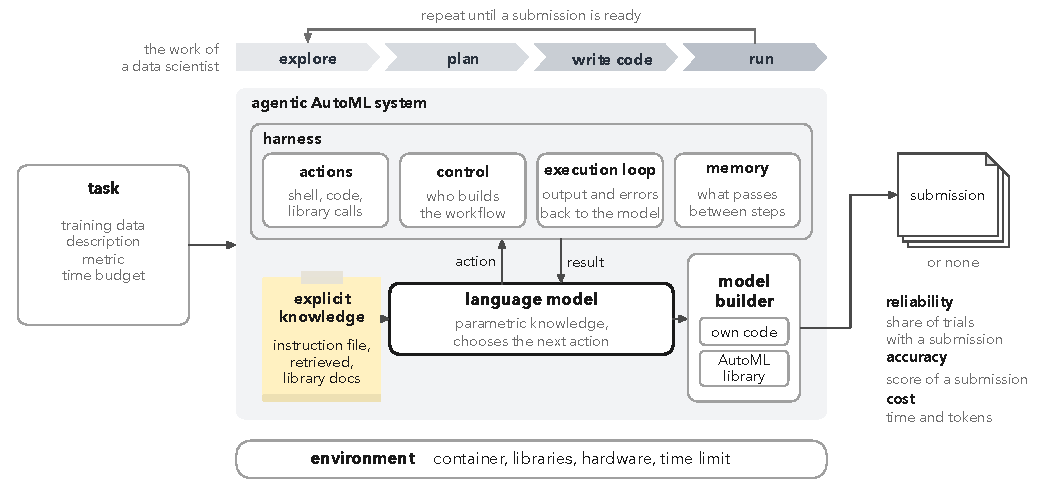
\includegraphics[width=\textwidth]{figures/fig_scheme.pdf}
\caption{The parts of an agentic AutoML system and the outcomes of a
trial. The thick outline marks the part that makes the decisions. Knowledge
about the procedure is held in four places: parametric knowledge in the
language model, the knowledge of the designers in the harness, knowledge
about search and tuning in the AutoML library, and explicit knowledge passed
to the model as text.}
\label{fig:scheme}
\end{figure*}
